\newcommand{\foo}{\hspace{-2.3pt}$\bullet$ \hspace{5pt}}

\begin{frame}
  \begin{center}
    {\color{Maroon}\Huge Introduction}
  \end{center}
\end{frame}

%% put section outline here
\begin{frame}{Introduction}{Outline}
  \begin{enumerate}
  \item The shift in speech based user interfaces
  \item Building applications on the information rich speech signal
  \item The Speech Recognition Case Study
    \begin{itemize}
    \item From rule-based systems to data-driven system
    \item Impact of speech recognition technologies across languages and domains
    \item What is under the hood for speech recognition technologies?
    \item Building various ASR module and the impact of data
    \end{itemize}
  \item Building ASR Systems in New Languages
    \begin{itemize}
    \item Building from ASR systems from scratch
    \item Is there room for sharing data from other languages?
    \end{itemize}
  \item Building ASR Systems in New Domain
    \begin{itemize}
    \item Adaptation of an existing ASR system
    \end{itemize}
  \end{enumerate}
\end{frame}

\begin{frame}{Speech based user interfaces}{}
\begin{columns}[T]
    \column{2.5in}
     \alert{Star Trek's Universal Translator} [Wikipedia] -  \dots used in the late 22nd century on 
     Earth for the \alert{instant translation of well-known Earth languages}. Gradually, with 
     the removal of language barriers, Earth's disparate cultures came to terms of 
     universal peace. Translations of \alert{previously unknown languages}, such as those of 
     aliens, required more difficulties to be overcome. 
     \column{2in}
     \vspace{1cm}
     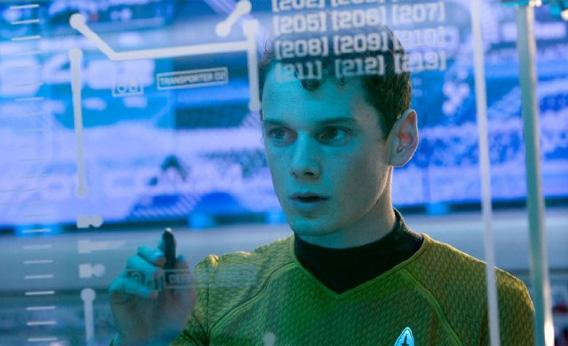
\includegraphics[height=30mm]{figures/startrek_comp}
  \end{columns}
\end{frame}

\begin{frame}{Speech based user interfaces}{}
\begin{columns}[T]
    \column{3in}
     \alert{Star Trek's The Next Generation Technical Manual} [Wikipedia] -  \dots the Universal Translator 
     is an "extremely sophisticated computer program" which functions by \alert{analyzing the patterns} of an unknown 
     foreign language, starting from \alert{a speech sample of two or more speakers in conversation}. The more extensive 
     the conversational sample, the more accurate and reliable is the "translation matrix," enabling instantaneous 
     conversion of verbal utterances or written text between the alien language and Federation Standard.
     \column{1in}
     \vspace{1.2cm}
     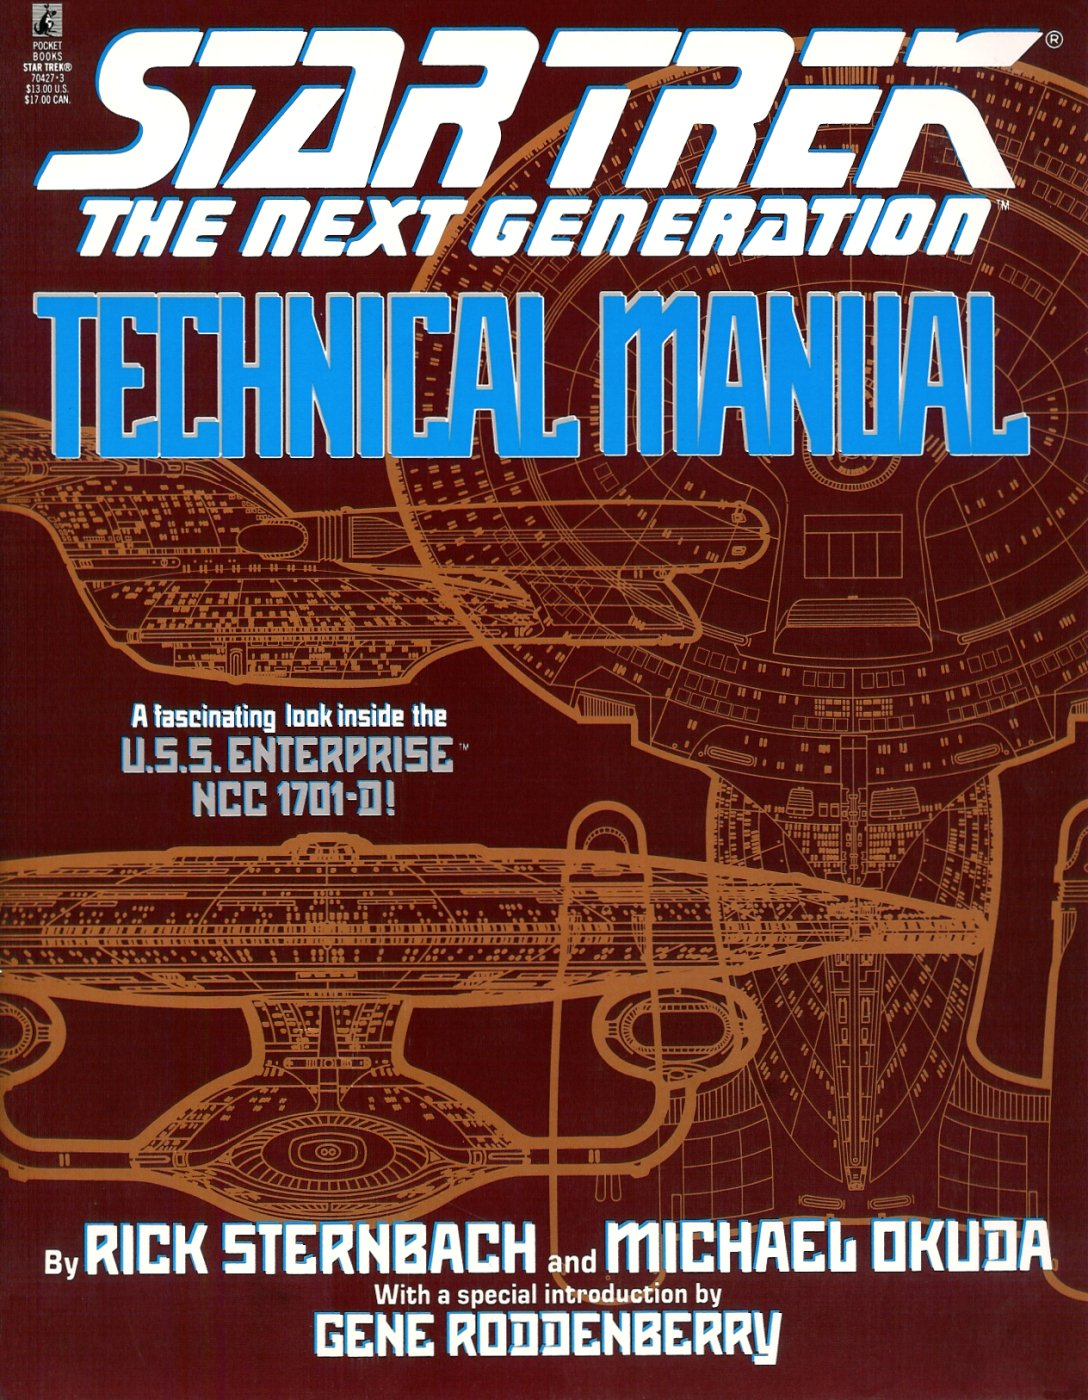
\includegraphics[height=40mm]{figures/startrek_manual}
  \end{columns}
\end{frame}

% Various applications that can be built on the speech signal
\begin{frame}{Building applications on the speech signal}
   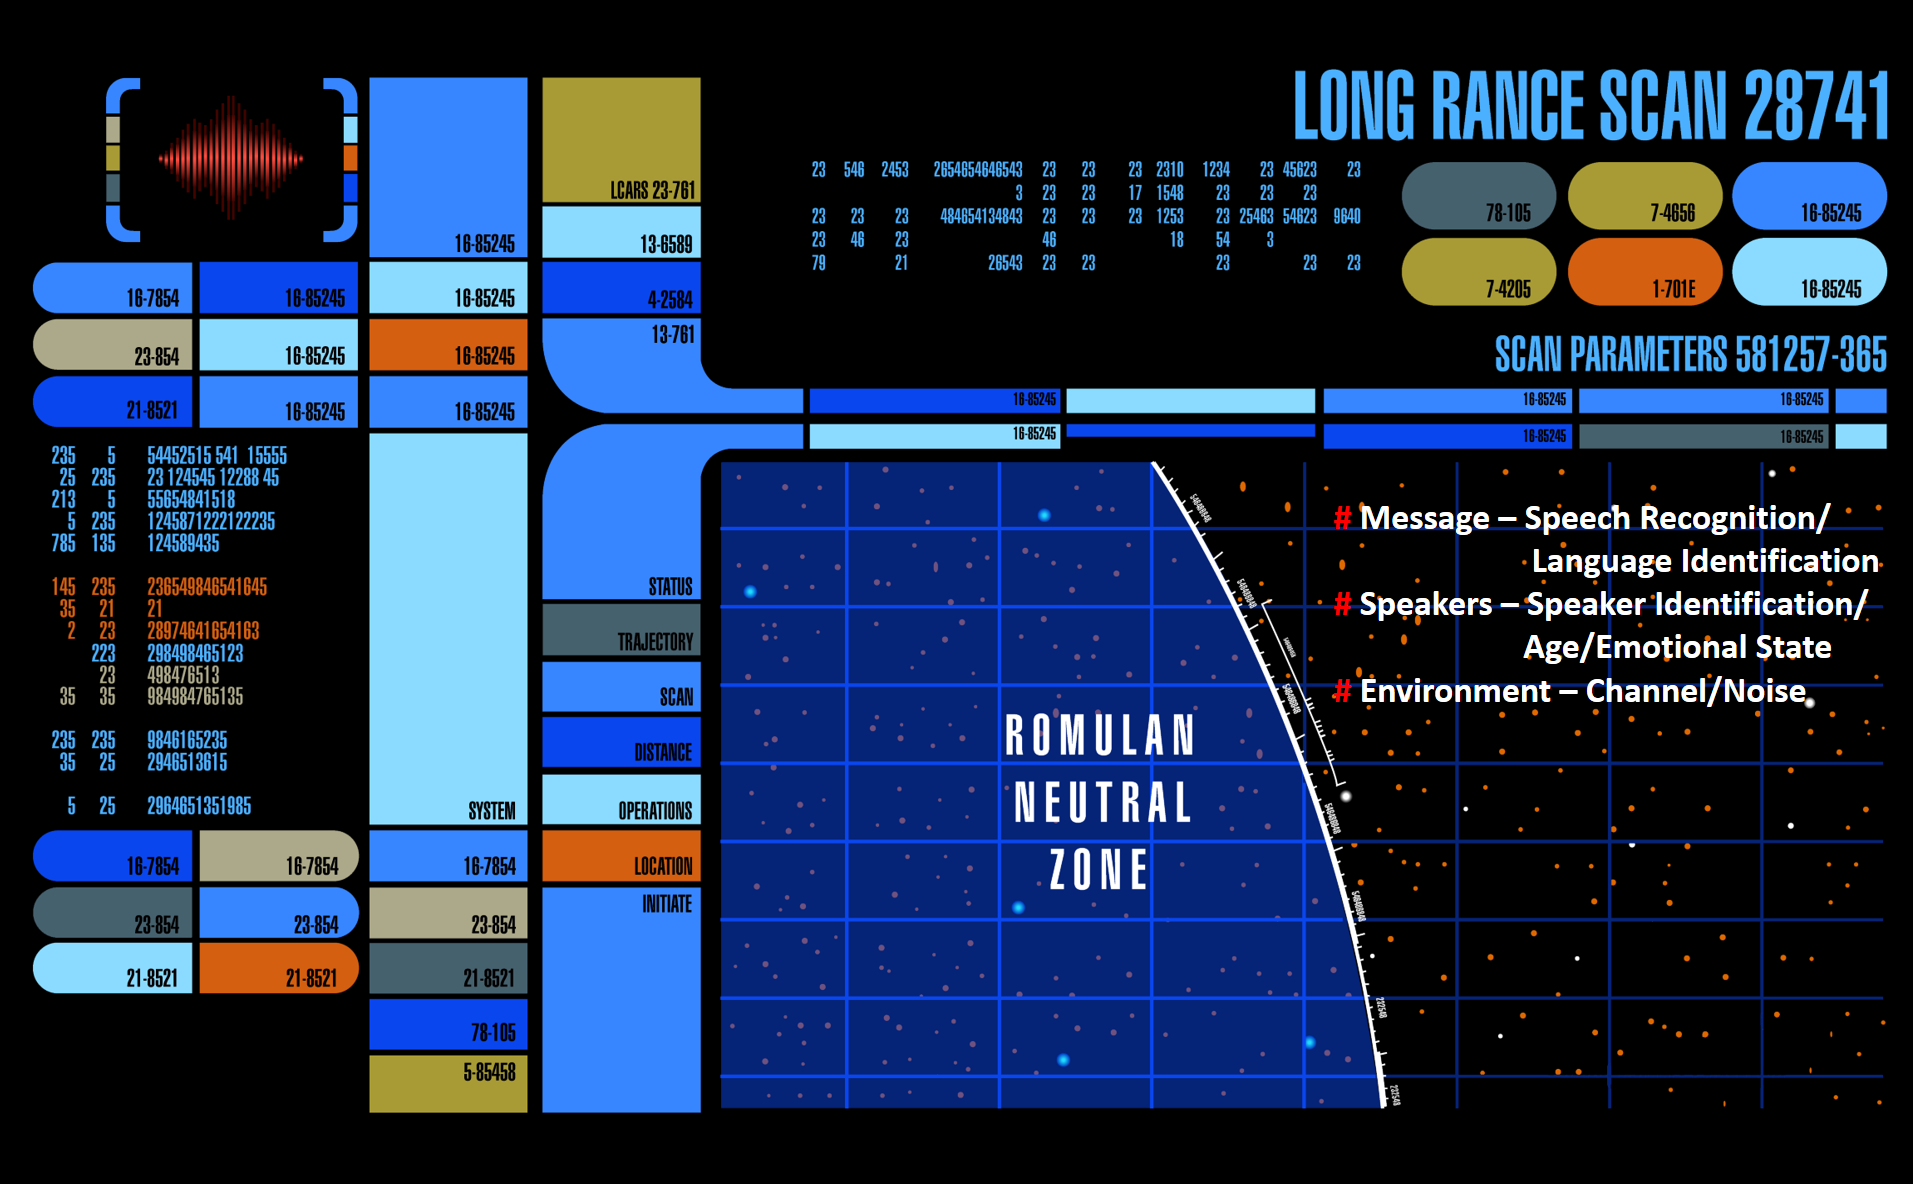
\includegraphics[height=70mm]{figures/technologies}
\end{frame}

% Show the progress from rule based to data based technologies
\begin{frame}{The march to becoming ubiquitous?}
\scalebox{1}{
\begin{tabular}{r |@{\foo} l}

{\color{red}1877} & Thomas Edison's phonograph\\
{\color{red}1936} & First electronic speech synthesizer - the Voder\\
{\color{red}1962} & IBM's Shoebox - understands up to 16 spoken\\
{\color{red}1976} & DARPA program - CMU's 1K word recognizer - Harpy\\
{\color{orange}1980} & HMMs - IBM's 20K word recognizer - Tangora\\
{\color{orange}1990} & Dragon Dictate, consumer based speech recognition\\
{\color{orange}1993} & CMU's Sphinx-II LVCSR system\\
{\color{orange}1996} & IBM's MedSpeak commercial LVCSR system\\
{\color{ForestGreen}2007} & Microsoft's Windows Vista with speech recognition\\
{\color{ForestGreen}2008} & Google's Voice Search for iPhone\\
{\color{ForestGreen}2011} & Apple's Siri \\
{\color{ForestGreen}2014} & Microsoft's Cortona/Amazon's Echo \\

\end{tabular}
}
\end{frame}

% Show the progress in building technolgies acorss languages
\begin{frame}{In how many different ways can we speak?}
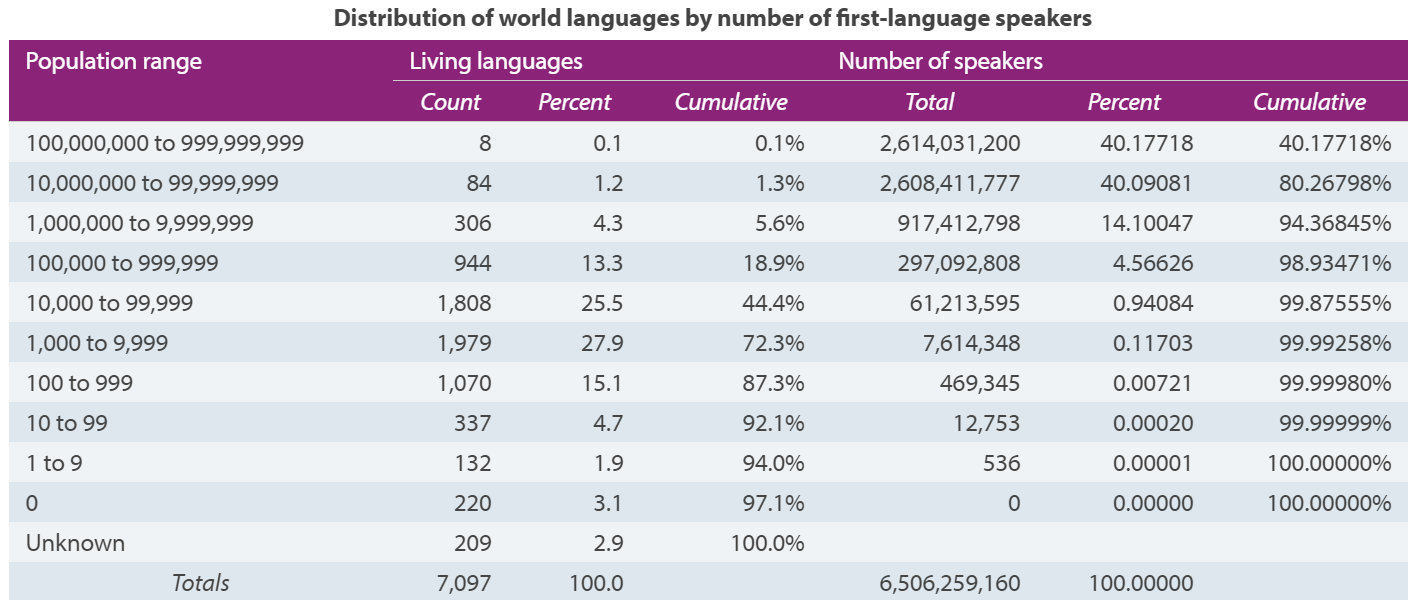
\includegraphics[height=48mm]{figures/languages}
\end{frame}

% Show the progress in building technolgies acorss languages
\begin{frame}{Do speech technologies stand tall?}
\begin{columns}[T]
    \column{1.4in}
     \vspace{2.5cm}
     \alert{Less than 4\%} of the language space has been covered!
     \column{2.8in}
     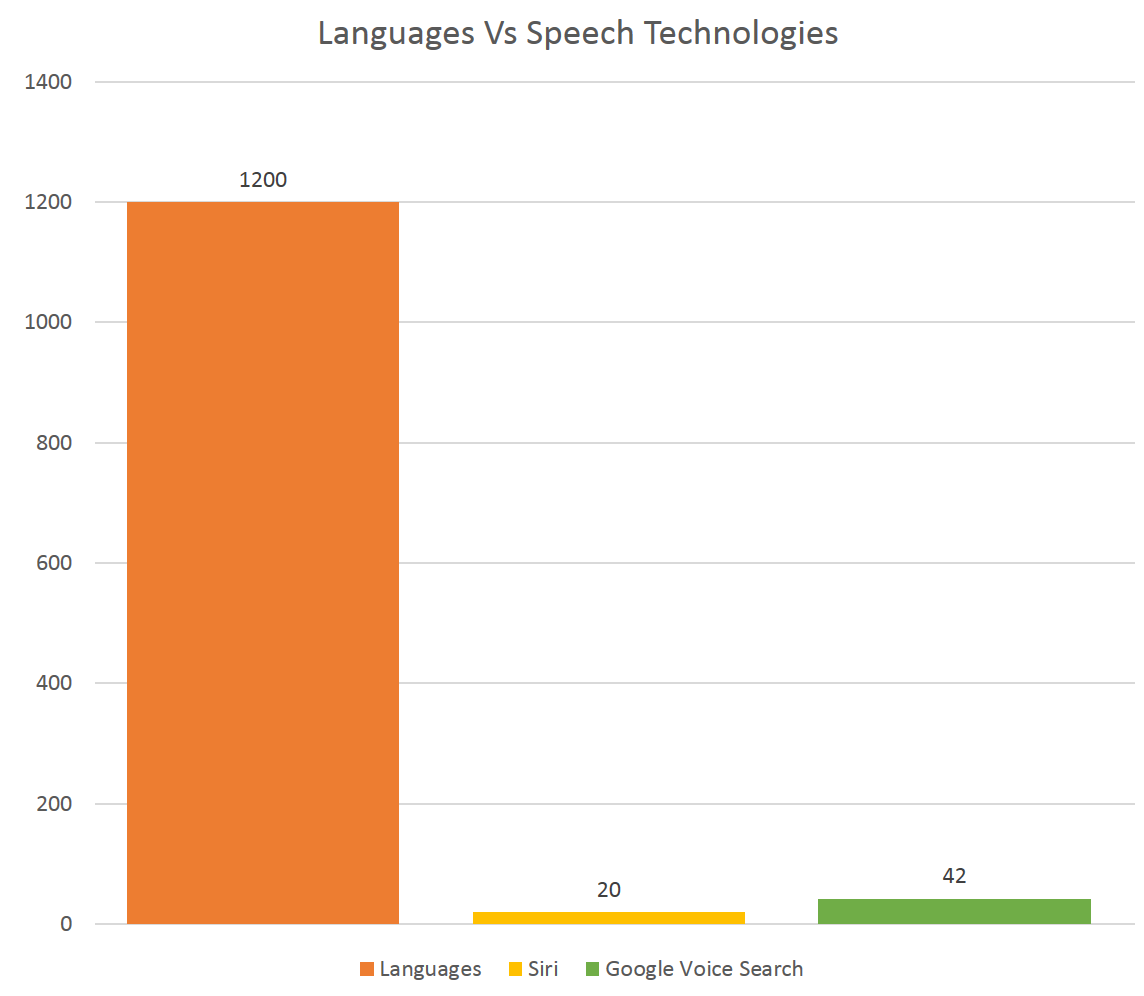
\includegraphics[height=68mm]{figures/lan_tech}
  \end{columns}
\end{frame}

% Show the progress in building technolgies acorss languages
\begin{frame}{For a given language, New Speech Applications = New Domains?}

\begin{enumerate}
\item Applications
\begin{enumerate}
  \item Mobile phone applications - voice search
  \item IVR applications/Call centers
  \item Dictation - Medical Transcription
  \item Surveillance - Military/Law enforcement
  \item In-car/at-home appliances
  \item Education/Accessibility
  \item Transcription - Court reporting
  \item Robotics/Gaming
\end{enumerate}
\item Noise distortions to speech input of existing applications
\begin{enumerate}
  \item Additive Noise
  \item Convolutive Noise
\end{enumerate}
\item Every new speech recognition deployment!
\end{enumerate}
\end{frame}

\begin{frame}{Dealing with New Languages and Domains}
\begin{columns}[T]
\column{2in}
\centering
{\color{orange}{New Languages}}
\begin{enumerate}
\item Every language is \alert{unique} although they might share many constructs with other languages
\item \alert{Seperate resources} specific to the language for building ASR systems are required,
possibility to share resources across languages
\item \alert{Building a new ASR system from scratch}
\end{enumerate}
\column{2in}
\centering
{\color{ForestGreen}{New Domains}}
\begin{enumerate}
\item Domains might have specific constructs but usually involves \alert{tailoring existing resources} of a language
\item Resources from the same languages can be \alert{shared}
\item Usually \alert{an ASR adaptation problem} rather than building from scratch
\end{enumerate}
\end{columns}
\end{frame}

\begin{frame}{What's under the hood for ASR?}
\begin{enumerate}
\item Automatic speech recognition is the process of transcribing speech into text
\item Speech recognition systems solve this task in a probabilistic setting using five key
components: a feature extraction module, an acoustic model, a pronunciation dictionary, a language model
and a search engine.
\end{enumerate}
\end{frame}

\begin{frame}{What's under the hood for ASR?}
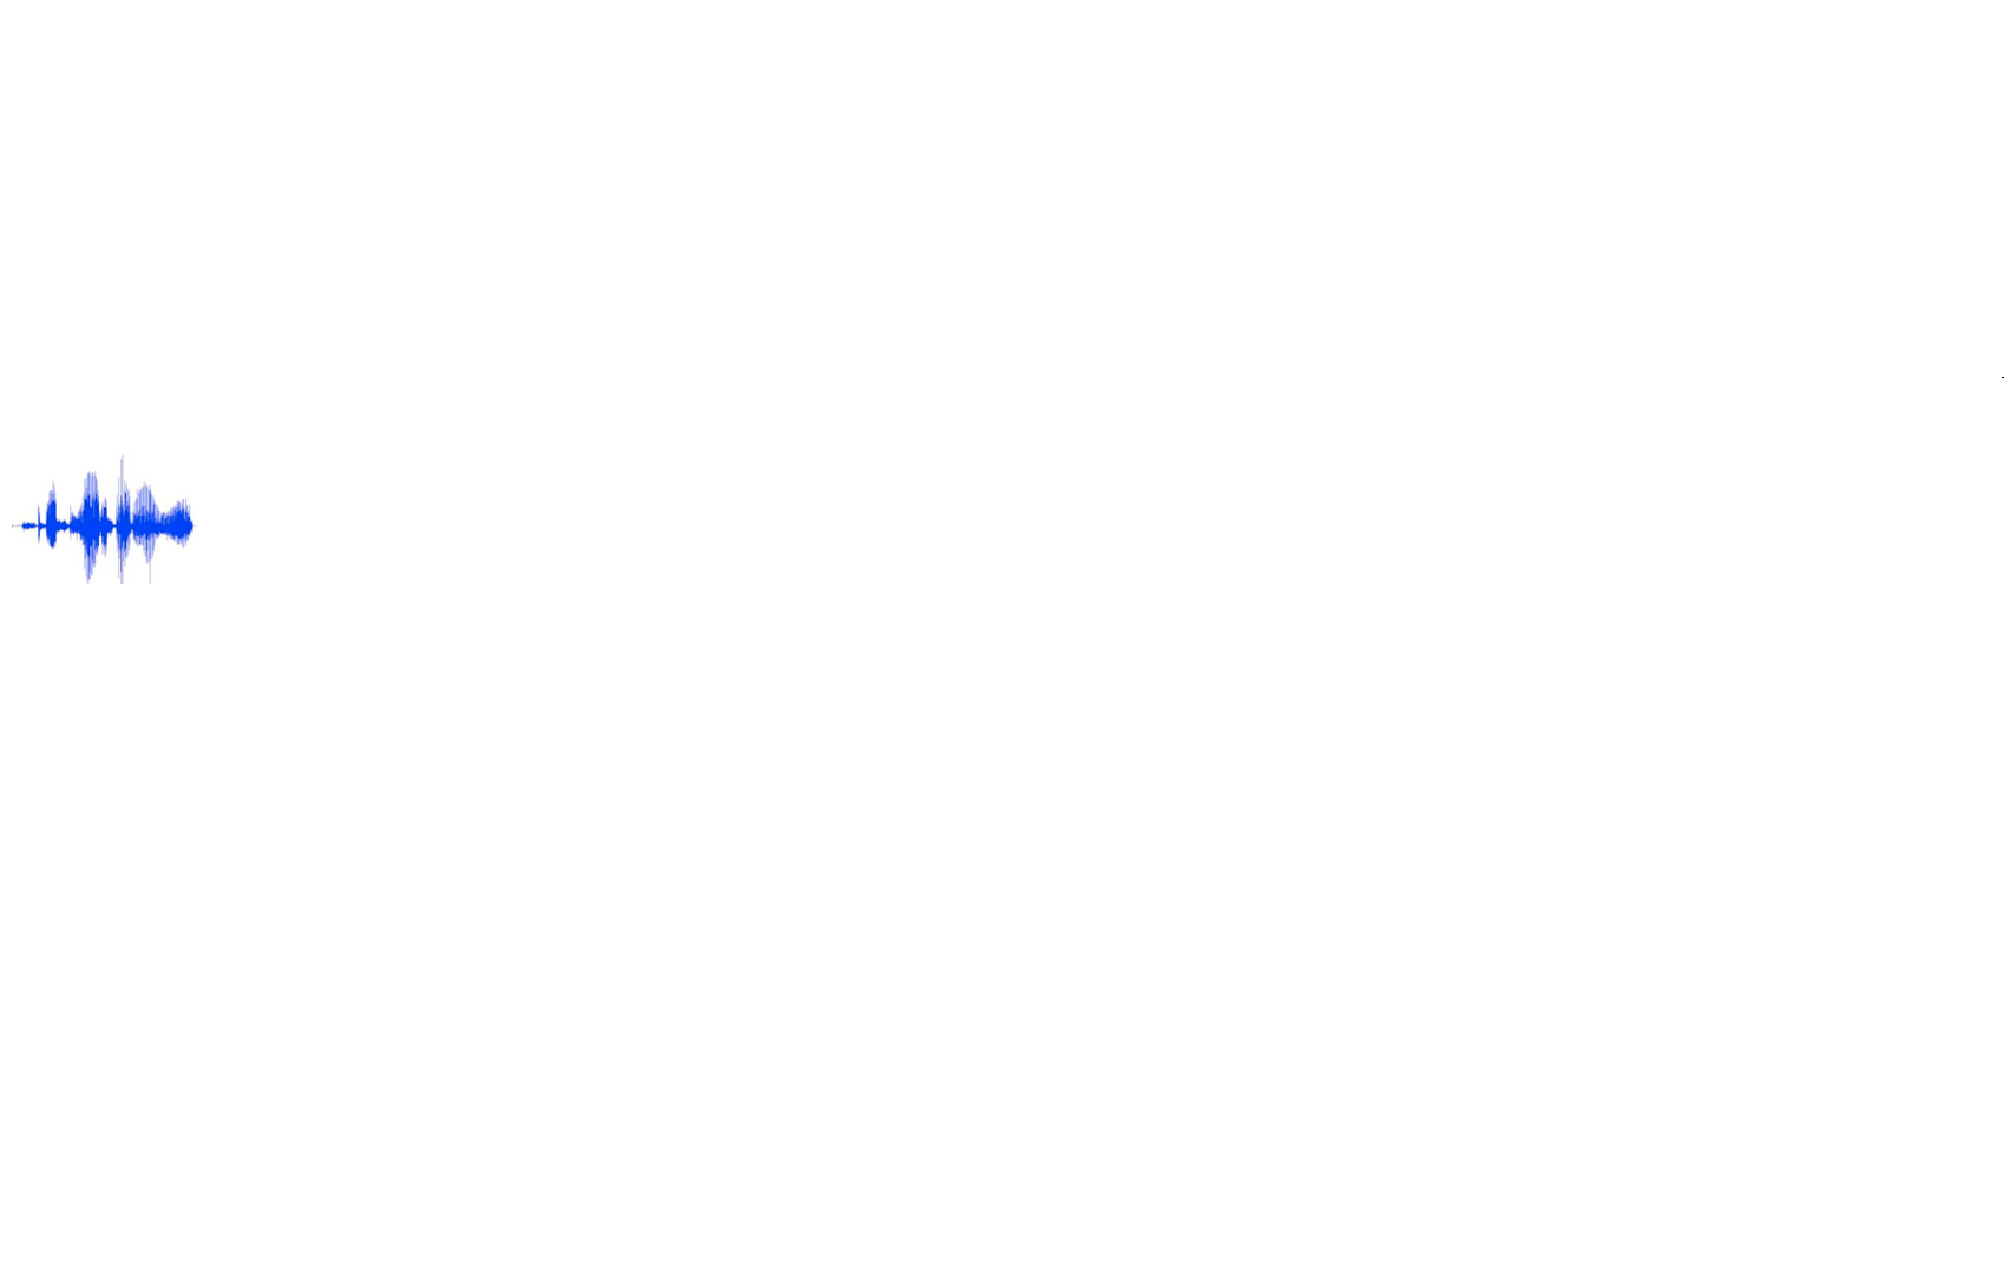
\includegraphics[height=70mm]{figures/ASR1}
\end{frame}

\begin{frame}{What's under the hood for ASR?}
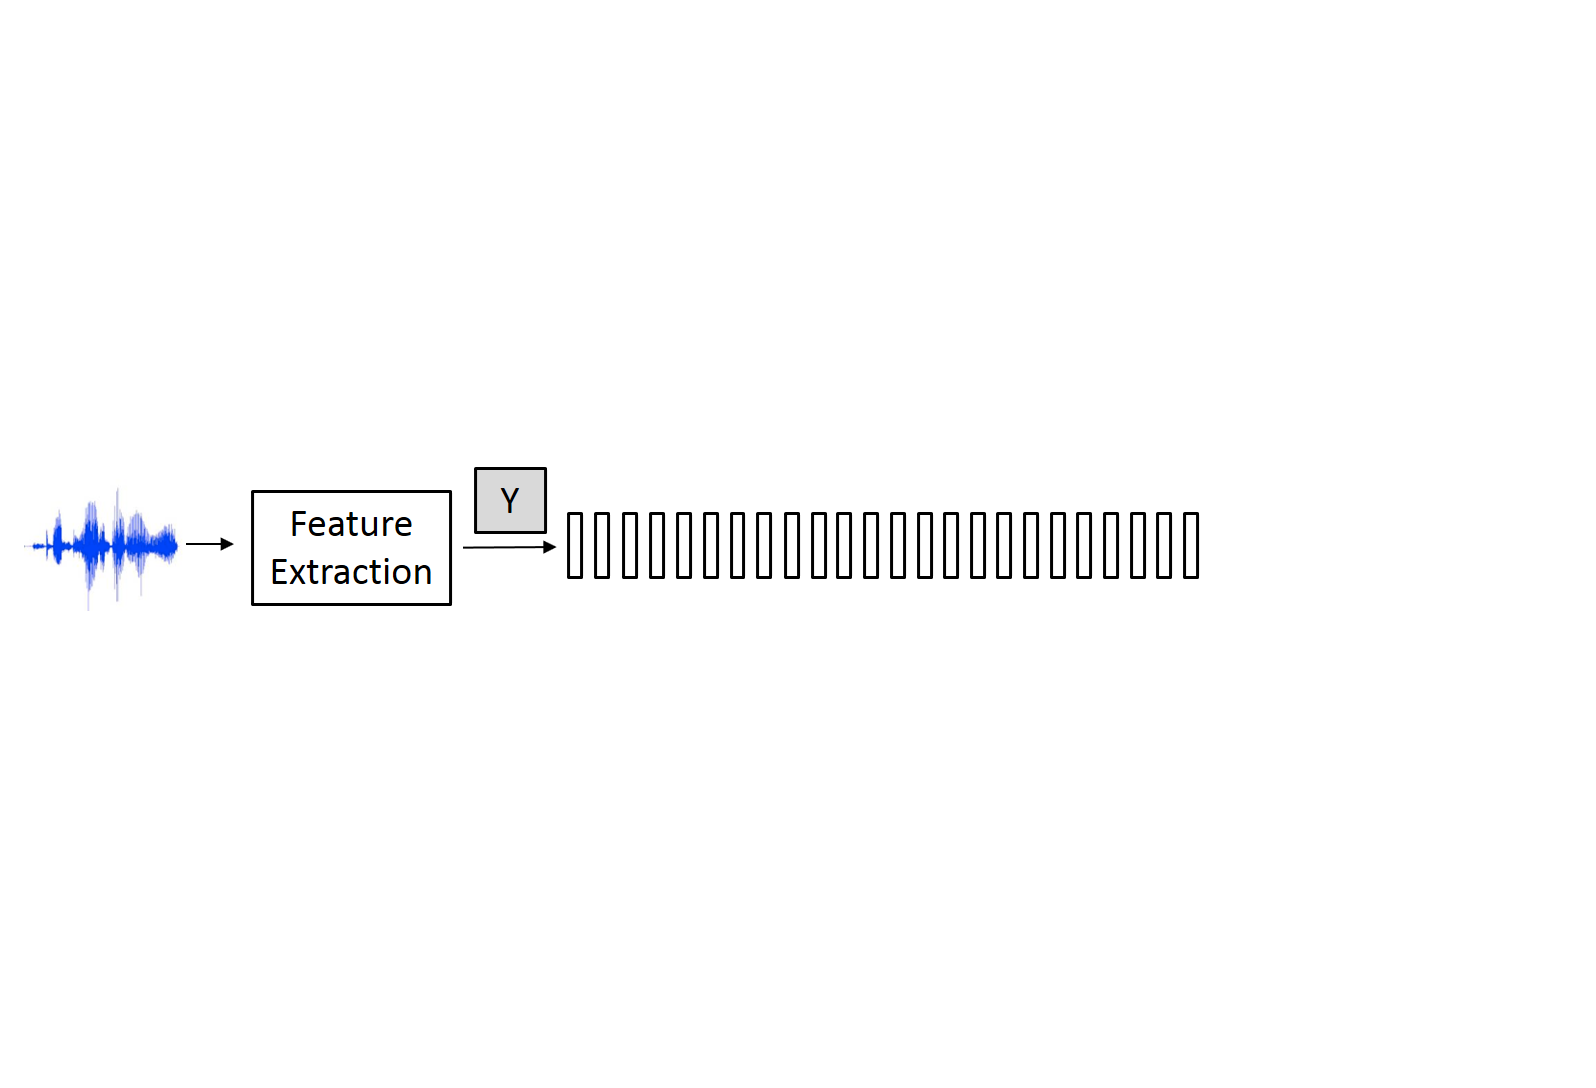
\includegraphics[height=70mm]{figures/ASR2}
\end{frame}

\begin{frame}{What's under the hood for ASR?}
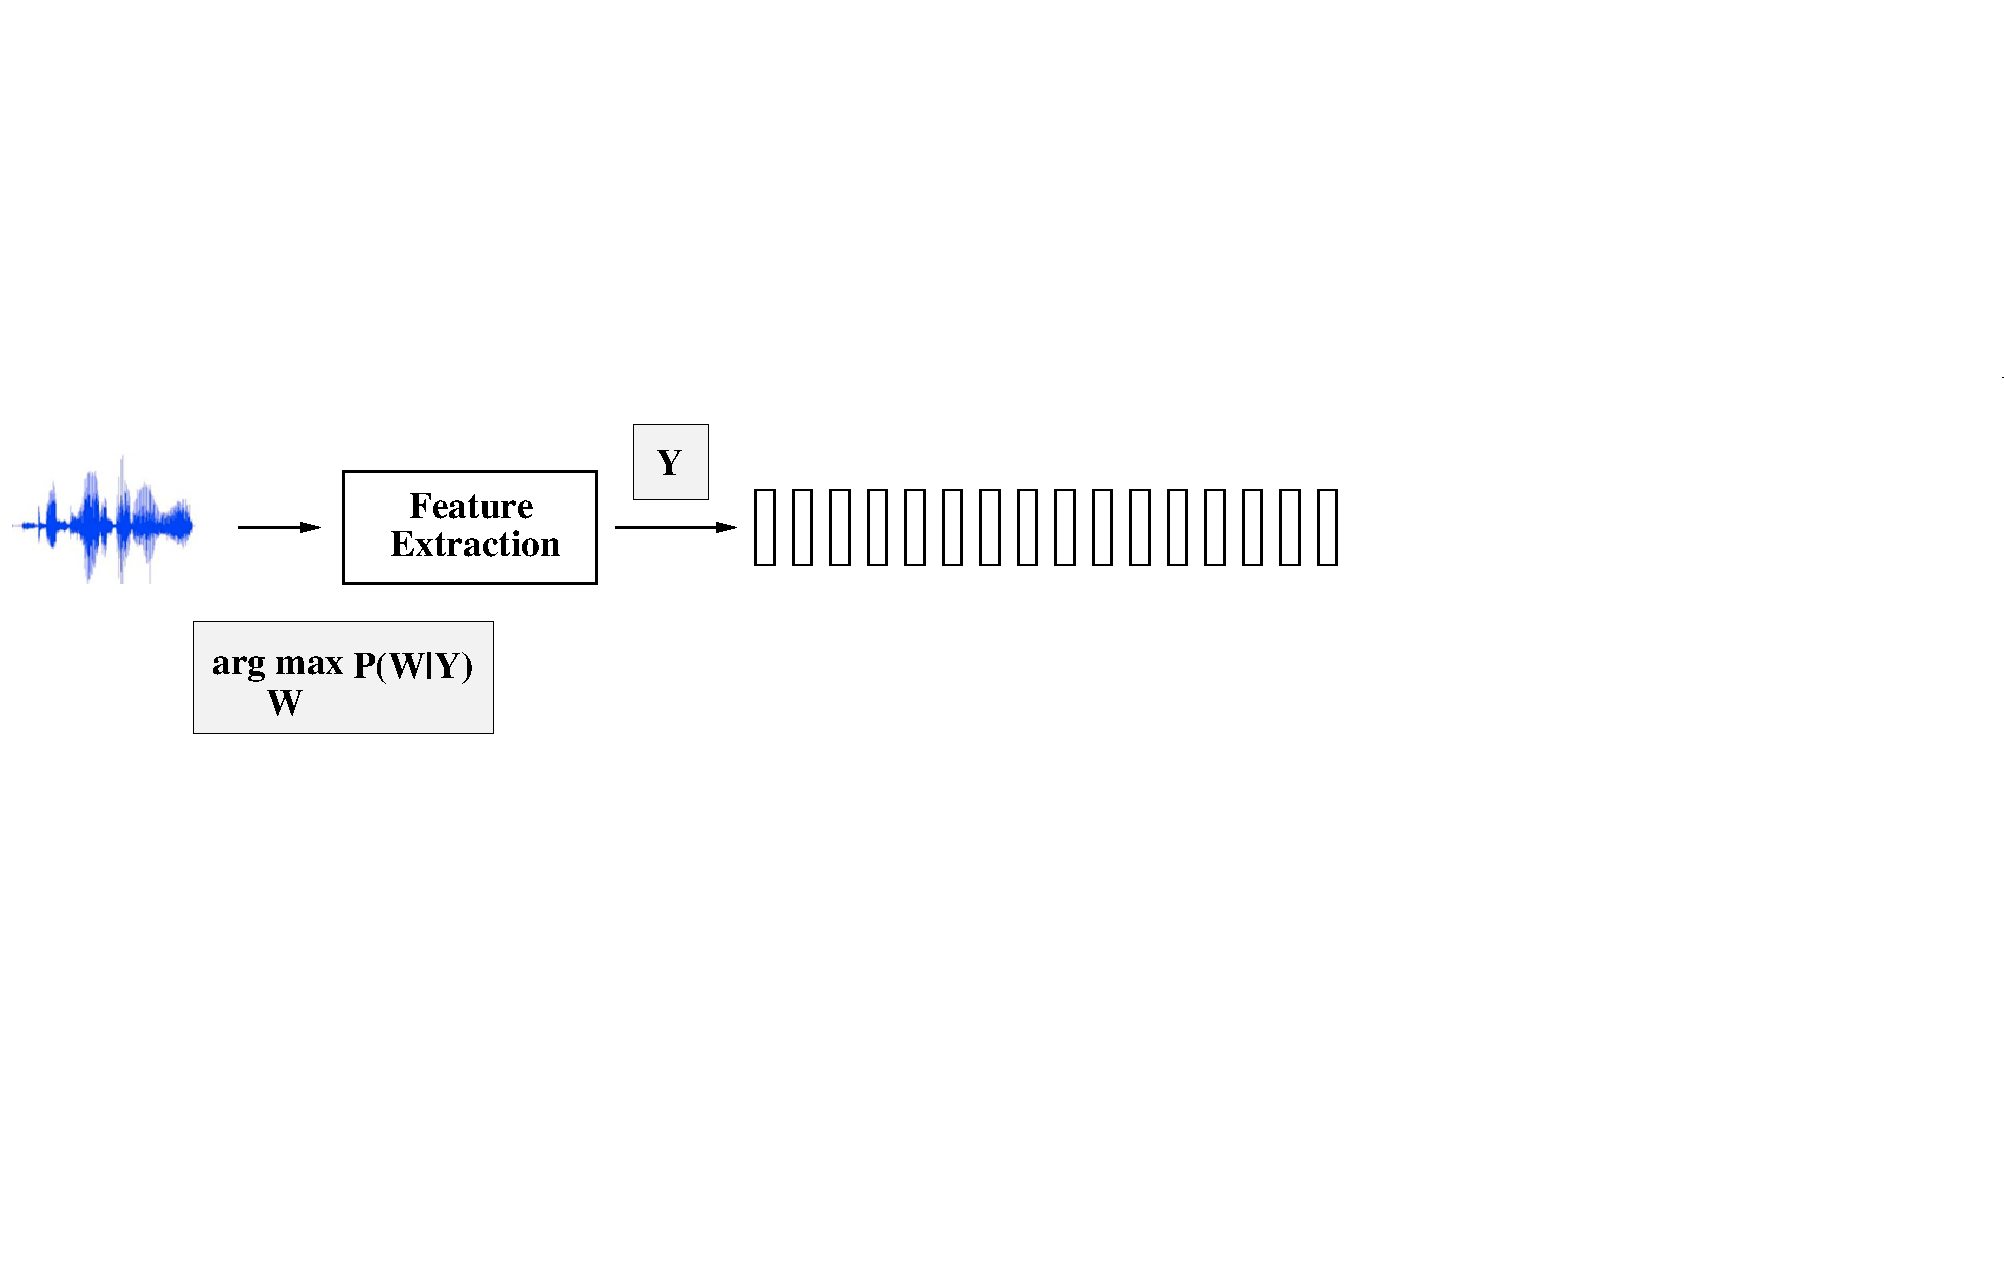
\includegraphics[height=70mm]{figures/ASR3}
\end{frame}

\begin{frame}{What's under the hood for ASR?}
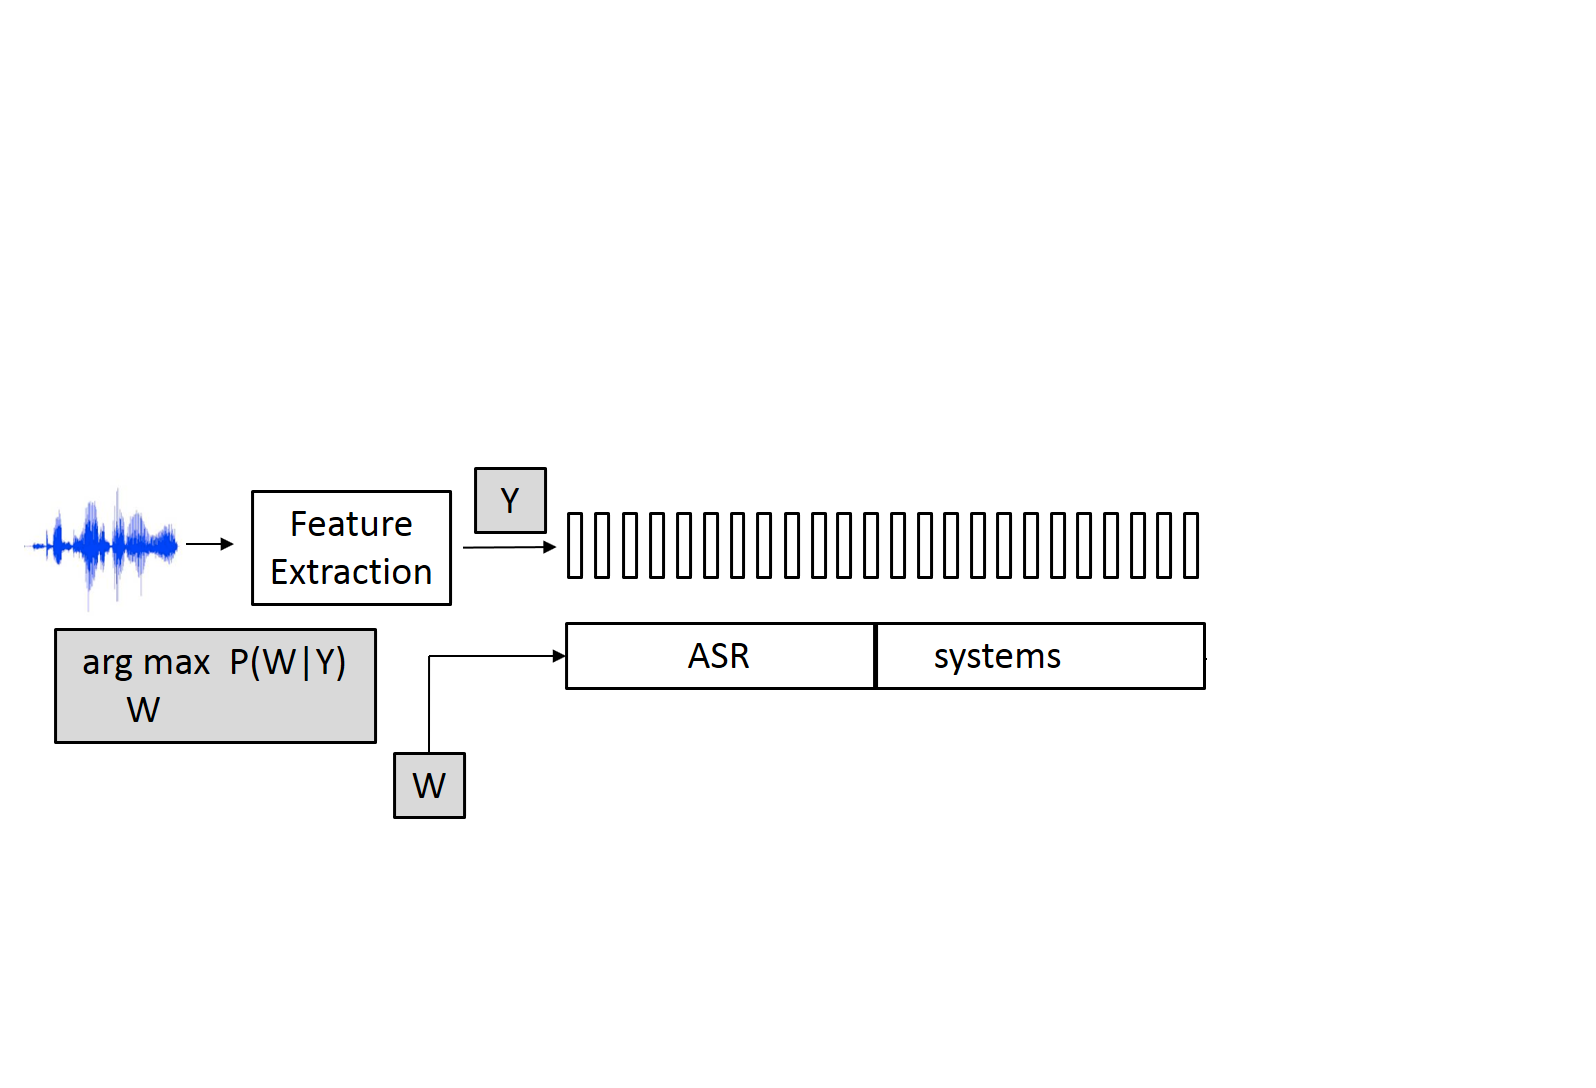
\includegraphics[height=70mm]{figures/ASR4}
\end{frame}

\begin{frame}{What's under the hood for ASR?}
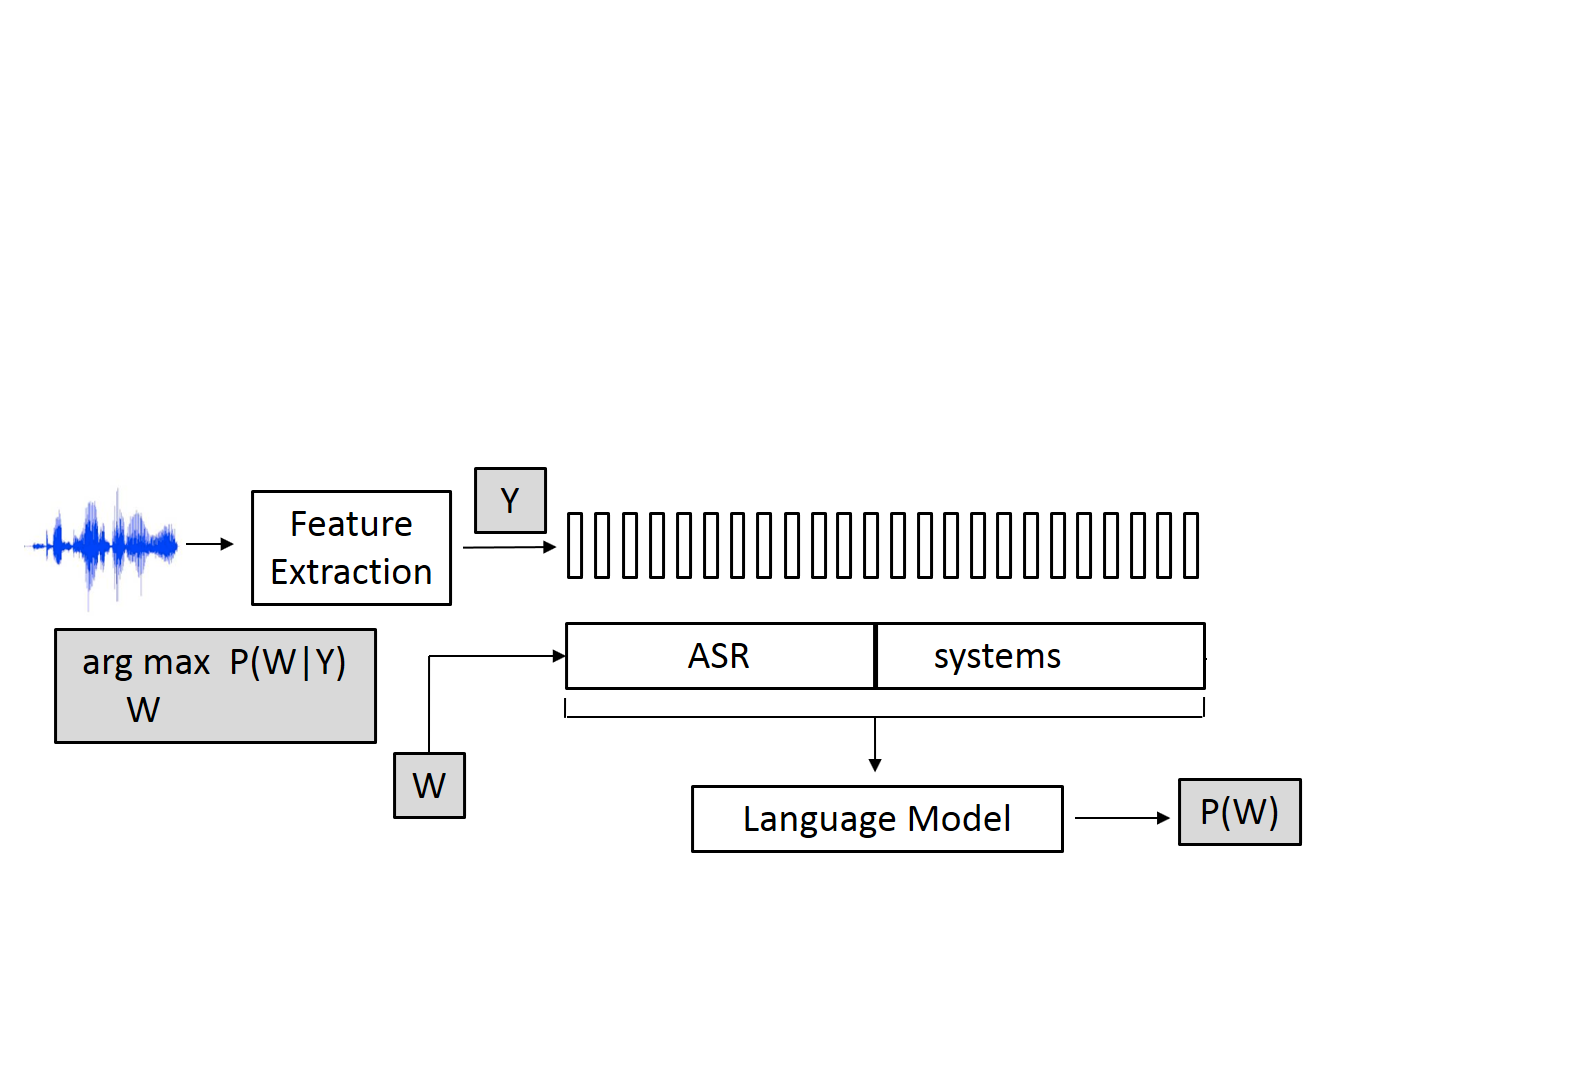
\includegraphics[height=70mm]{figures/ASR5}
\end{frame}

\begin{frame}{What's under the hood for ASR?}
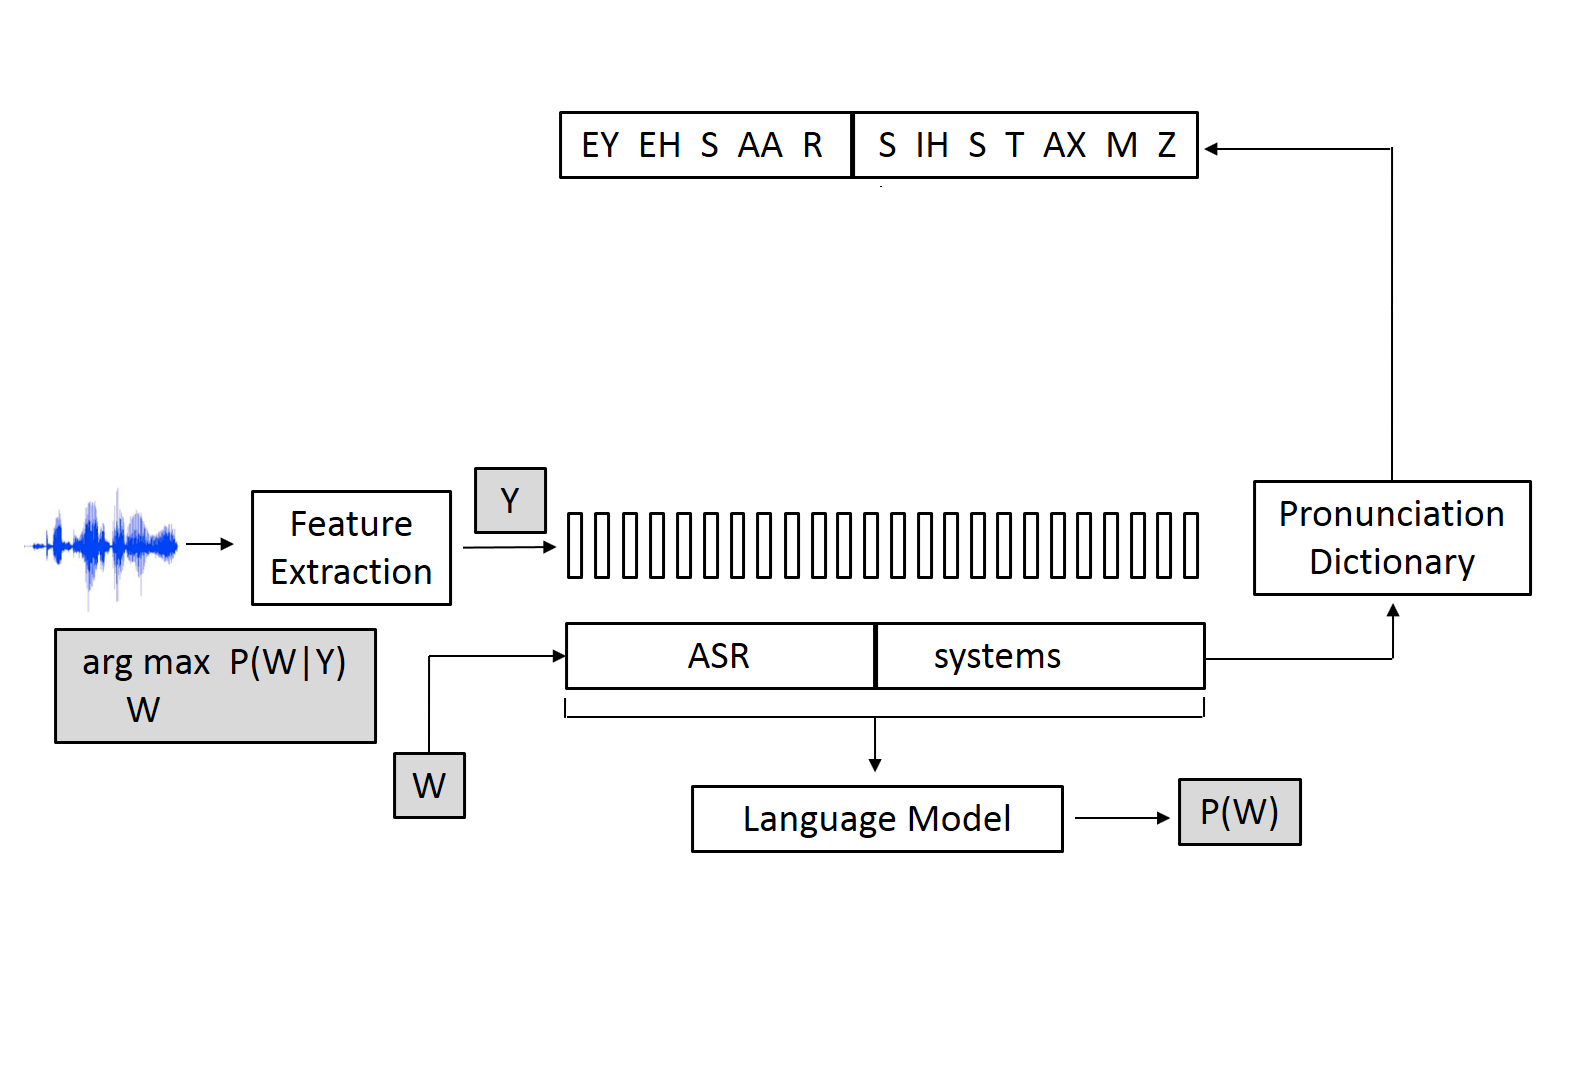
\includegraphics[height=70mm]{figures/ASR6}
\end{frame}

\begin{frame}{What's under the hood for ASR?}
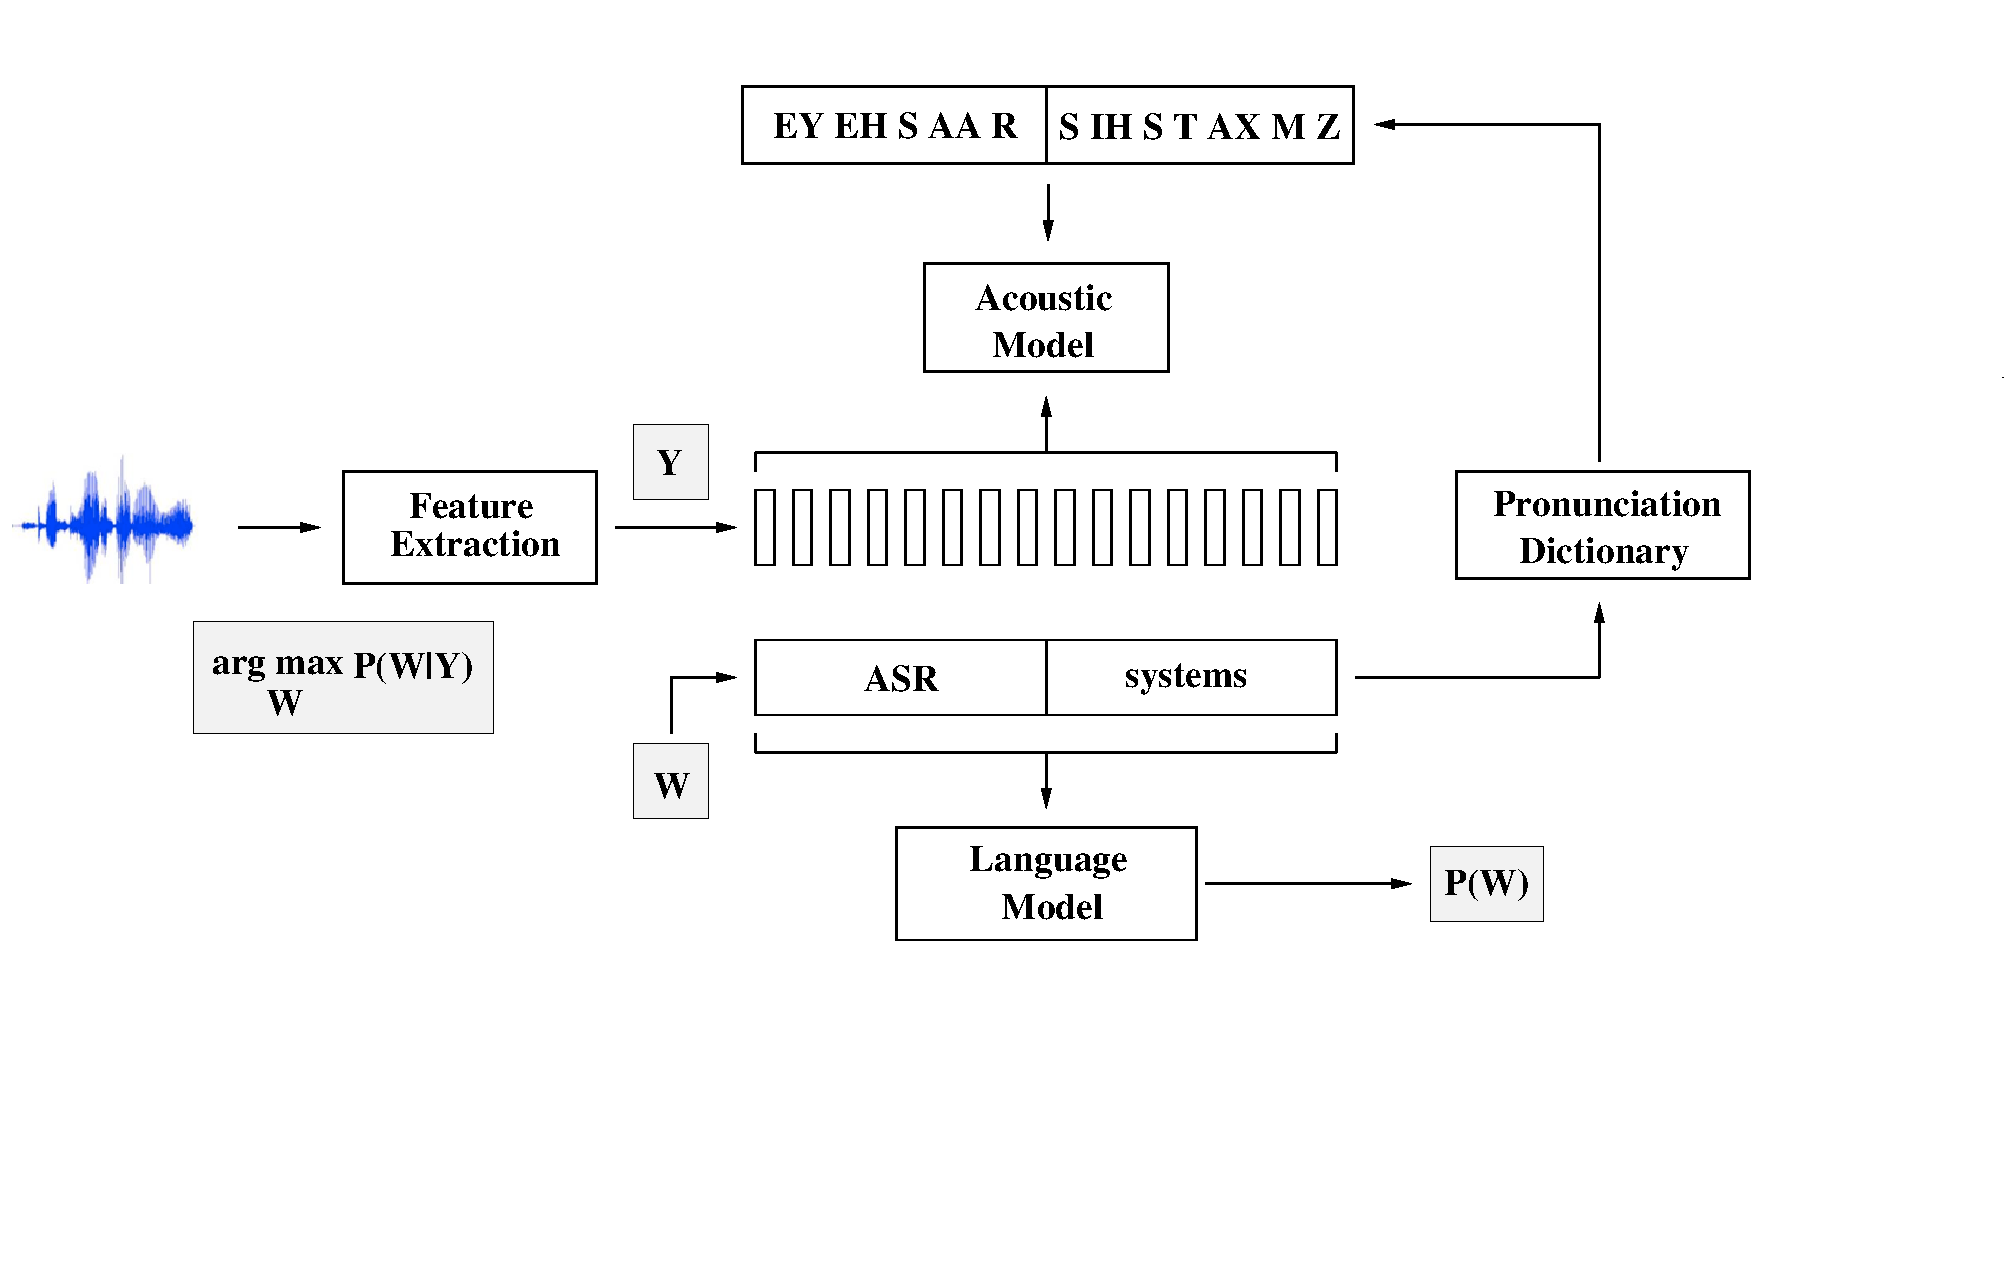
\includegraphics[height=70mm]{figures/ASR7}
\end{frame}

\begin{frame}{What's under the hood for ASR?}
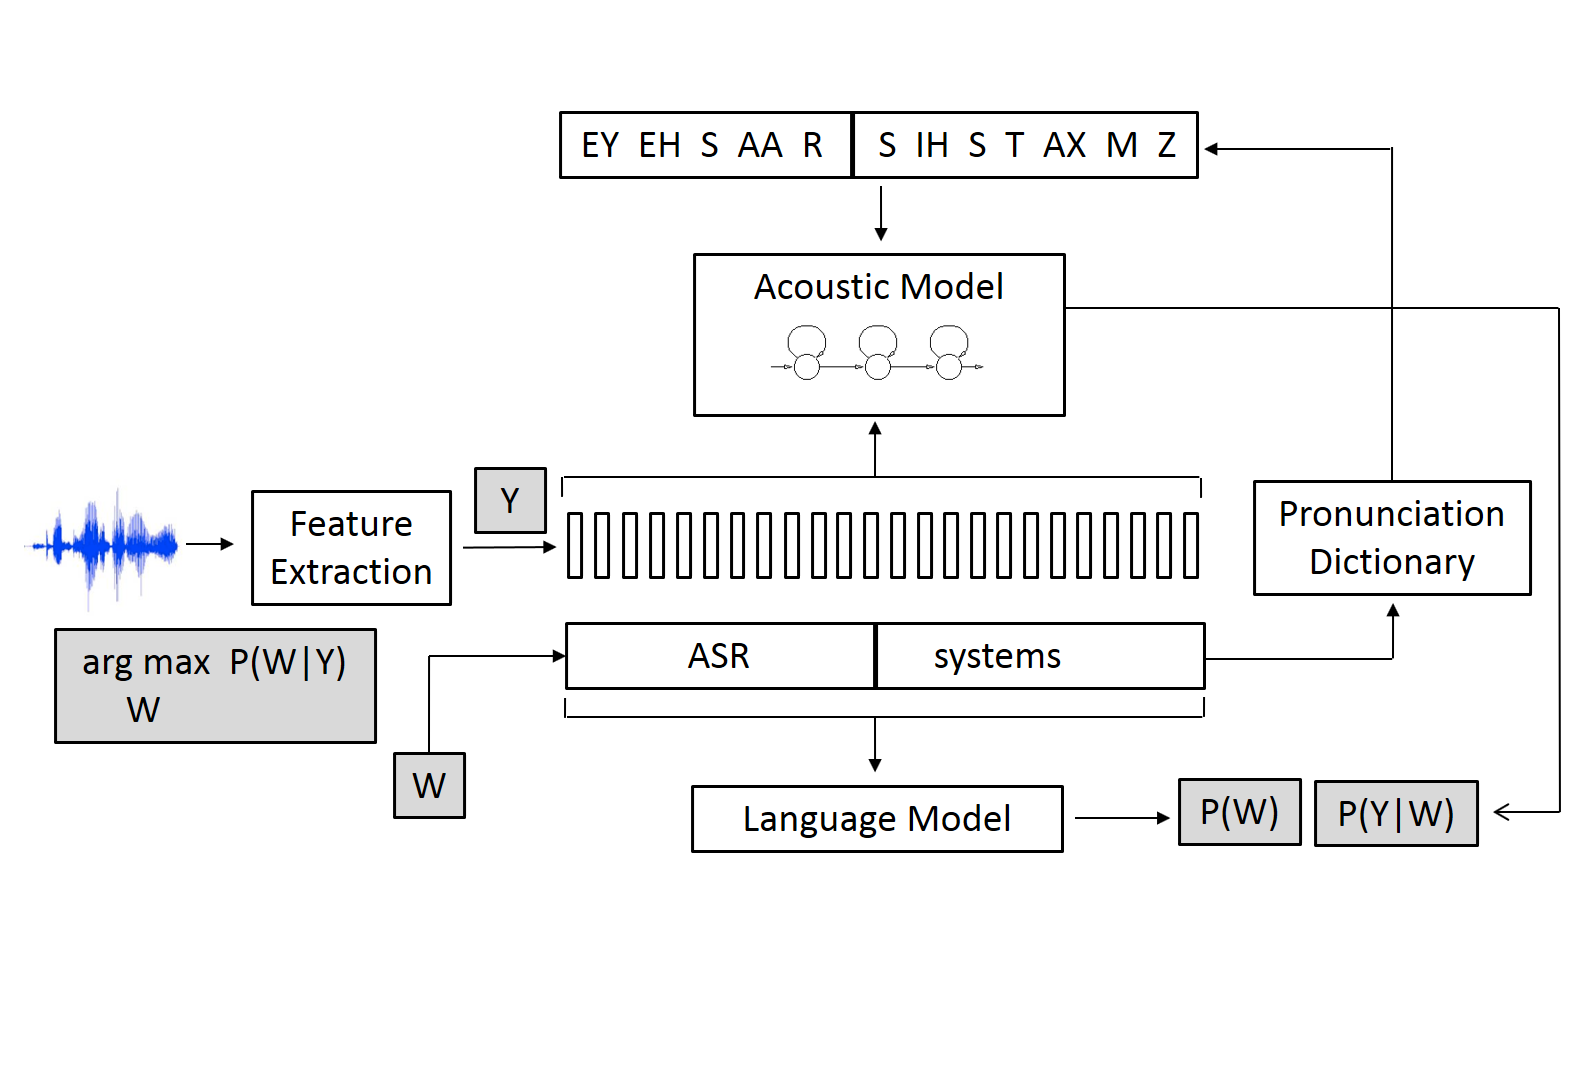
\includegraphics[height=70mm]{figures/ASR8}
\end{frame}

\begin{frame}{What's under the hood for ASR?}
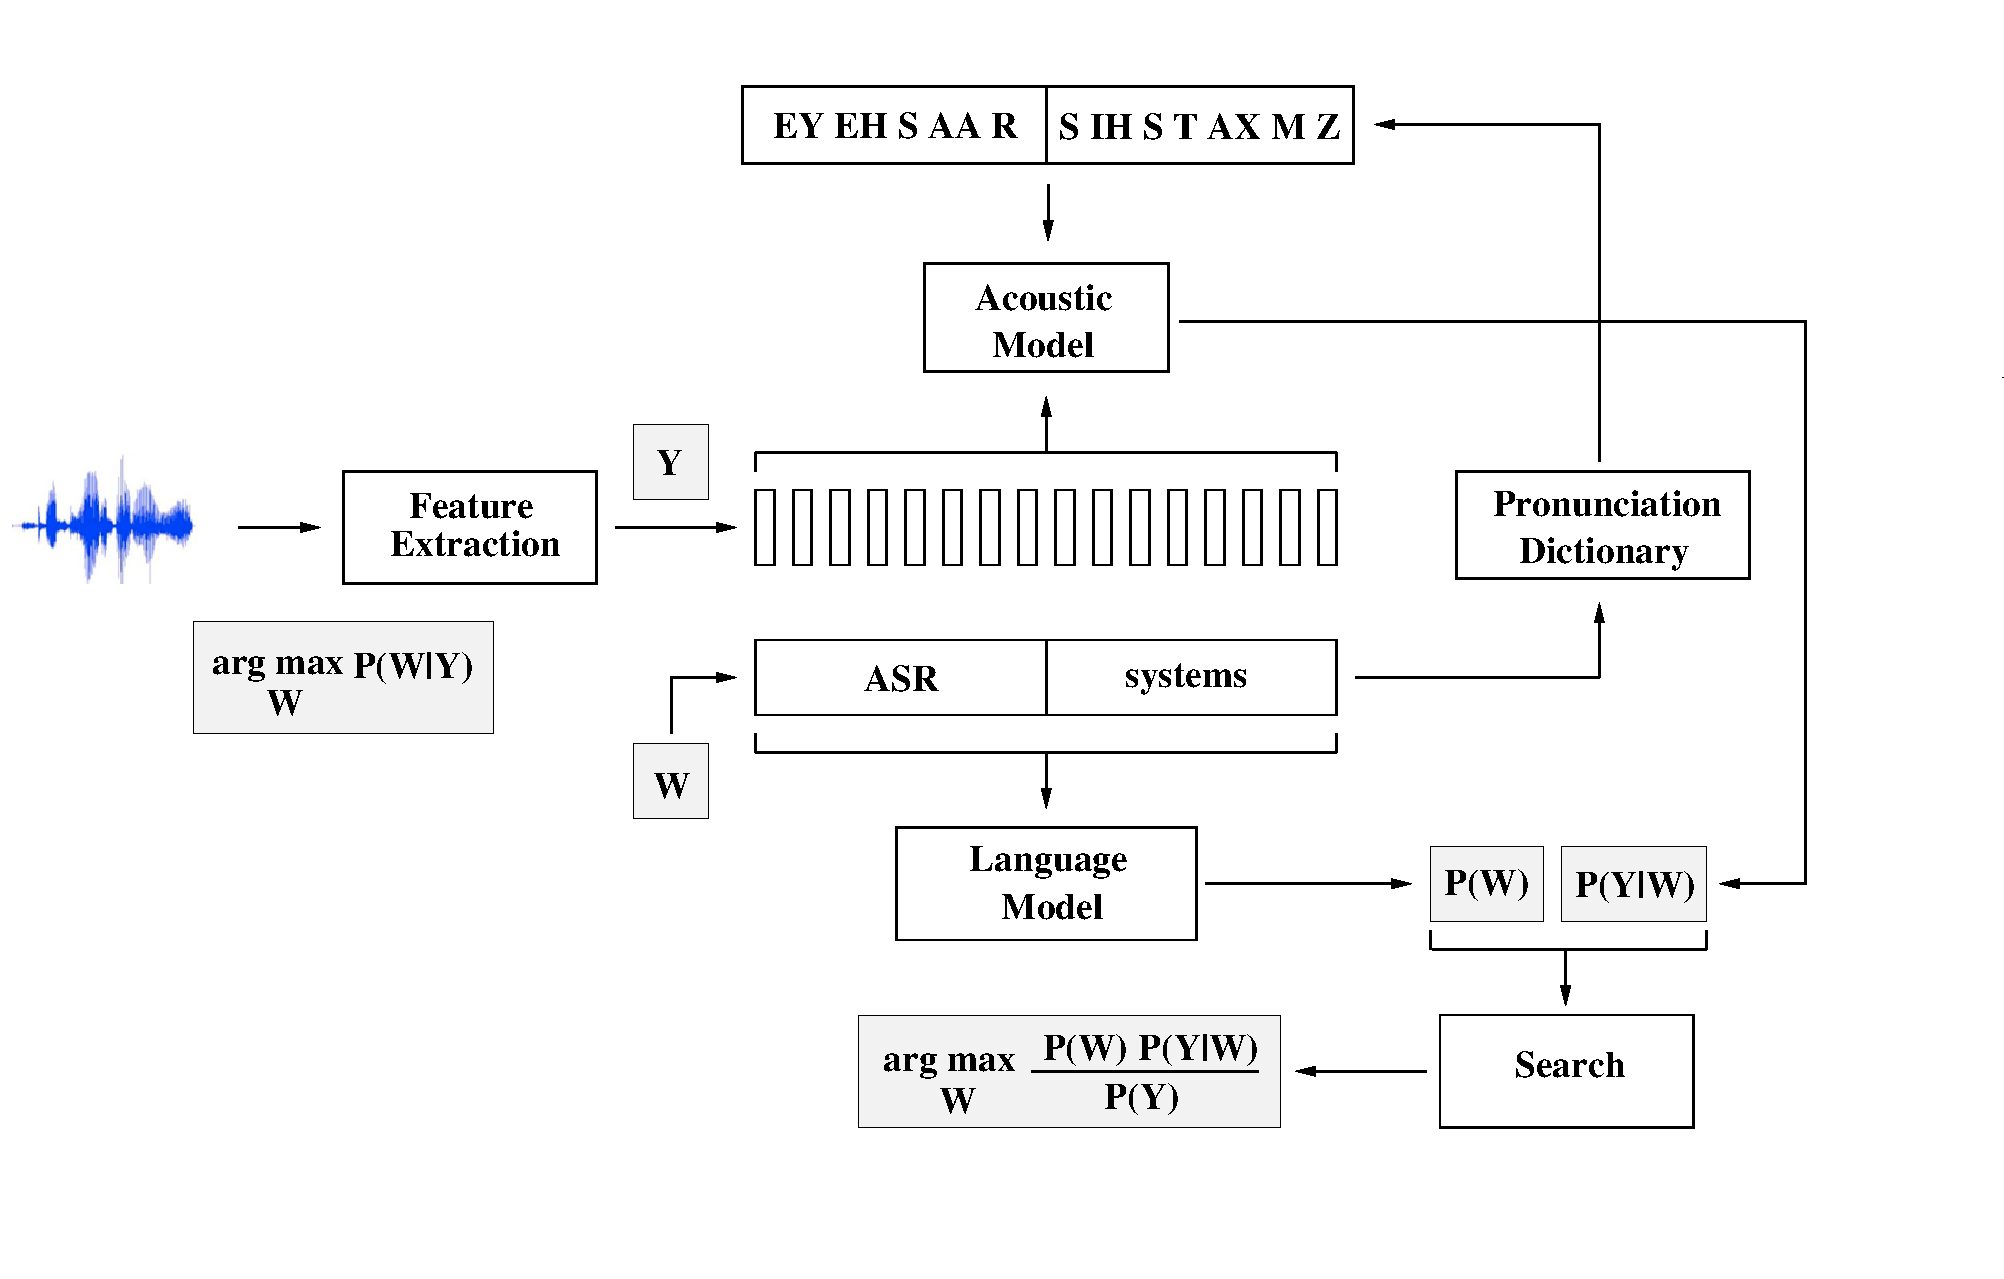
\includegraphics[height=70mm]{figures/ASR9}
\end{frame}


